\chapter{\label{ch:human_torso_model}Human Torso Model}
Our work is at the border between physical modelling, simulation in computer animation and related areas of interest such as physiology, anatomy, biomechanics and control. This chapter reviews relevant prior work on modelling and simulating the human torso, then describes the different mechanisms involved in breathing in order to explain how we modelled the rigid-parts of our simulation.

% -------------------------------------------------------------
% Section
% -------------------------------------------------------------
\section{\label{sec:related_work}Related work}
In previous work, human torso models have been simplified to a few components. For instance, Carranza et al. \cite{carranza2003free} uses a simple body model based on a triangle mesh shape and a kinematic skeleton. Others, such as Monheit and Badler \cite{monheit2002kinematic}, present a kinematic model of the human spine and torso where the total bending angle is distributed to each joint according to weighting parameters.

Lee et al. \cite{lee2009comprehensive, lee2008biomechanical} describes a detailed model of the whole upper body. The model derives from a musculoskeletal system with 814 Hill-type muscle actuators (a spring and a damper in parallel with another spring) and a coupled finite element simulation of soft tissue deformations. The skeleton is made of 68 bones. Using a commercial model called the Ultimate Human model \cite{ultimatemodel2008}, the team built the skeletal muscles using piecewise line segments. They omitted the diaphragm and as a result, the respiratory movement is mainly accomplished by the intercostal muscles. However, Konno et al. \cite{konno1967measurement} experimentally found that the abdomen accounted for around half of the tidal volume (volume of air displaced between normal inspiration and expiration) and just less than half of the vital capacity (maximum amount of air a person can expel). As a consequence, the role of the abdomen is absolutely crucial in breathing and its absence in \cite{lee2009comprehensive, lee2008biomechanical} makes the model incomplete in terms of breathing simulation. For model simplification reasons also, some muscles involved in breathing such as the transversus abdominis were avoided too. Special care is taken to model the soft tissue, as the goal sought here is to get a high quality surface representation from the model. To animate the model the authors use a two-step process: first they collect the different positions, orientations and joint angles of the main limbs of the upper body over time---from target key poses or motion capture data---and then they compute the muscle activation levels that have to be applied to the model in order to achieve these positions. Given the positions of the bones and the activation level of each muscle, the soft tissue is deformed according to coupling relations (linking bones and soft tissue, muscle forces and directions). Some simulations of breathing are presented in \cite{lee2009comprehensive} but the very few respiratory muscles used and the absence of abdominal breathing over-simplify the complex process of breathing and produce good but not totally realistic movements.

The models of the human torso presented by DiLorenzo et al. \cite{dilorenzo2008laughing, dilorenzo2009breathing} (known as the Breathe Easy model) and by Veltkamp et al. \cite{veltkamp2009physiological} use both anatomical and physical data to describe breathing. Using spring-based muscles the torso model can be put into motion by stimulating the ribs and the diaphragm (the abdomen and the gut move passively). The simulation also uses estimated pressure forces to preserve the volume of the deformable components such as the gut, which is modelled as a deformable and incompressible volume. They applied different contraction input signals and chose the most visually pleasing ones in their simulations. The authors derived their model from an existing skeleton available at \url{www.3Dcafe.com}, a free 3D database platform. However, the origin of the model used is unknown and no validation of its anatomical accuracy has been carried out.
In the Breathe Easy model, the skin surface is a NURBS\footnote{Non-Uniform Rational B-Spline.} surface based on trace vertices from the skeleton simulation; all the computation is done through the 3D modelling software program Autodesk Maya \cite{maya2010}. The validation of the model involved computing different volumes of the lung cavity of the model during different kind of breathing styles and to compare them to average figures that can be found in the literature. However, the volume curves shown in \cite{dilorenzo2008laughing} are not realistic according to \cite{veltkamp2009physiological}. Moreover, as the accompanying video of \cite{dilorenzo2008laughing} shows little abdominal breathing, \cite{veltkamp2009physiological} criticises the lack of realism of the simulation.

While \cite{nakamura2005somatosensory, zordan2004breathe, dilorenzo2008laughing, veltkamp2009physiological} present detailed models of the human torso, we note that important simplifications are used and particularly, the articular bones in the spine and the rib cage are grouped and treated as a single rigid body. In addition, the models presented by \cite{zordan2004breathe, dilorenzo2008laughing, veltkamp2009physiological} are put into motion by activating groups of muscles evenly, which is a simplification compared to the model we present in later chapters, in which activation inputs are fully tunable.

Finally, the only means of validation used in previous work relied on the plausible shapes of the curves obtained through simulation. In order to validate our method, we compare the simulation data to spirometry data.

% -------------------------------------------------------------
% Section
% -------------------------------------------------------------
\section{\label{sec:breathing_mechanisms}Breathing mechanisms}
To understand the different modelling decisions we made to build our torso simulation, we must first understand how humans breathe. This section describes the different breathing mechanisms and uses several medical terms which are defined here:

\begin{description}
	\item[caudal direction:] towards the tail end of the body.
	\item[cranial direction:] towards the head end of the body.
	\item[dorsal direction:] the surface directed towards the back or spine.
	\item[medial direction:] towards the median plane (a vertical plane passing through the body from nose tip to tail tip).
	\item[lateral direction:] the surface directed away from the median plane.
	\item[ventral direction:] the surface directed towards the belly or ground.
	\item[chondrocostal:] pertaining to the ribs and the costal cartilages.

\end{description}

Breathing is the process that moves air in and out of the lungs. The movement of breathing can be split into two distinct steps: inspiration and expiration. Inspiration consists of filling up the lungs with fresh air, rich in oxygen, by expanding the volume inside the chest wall. The oxygen is then transmitted to the blood through lung capillaries and is distributed to the whole body via the circulatory system. Meanwhile, through the same capillaries, the blood passes the carbon dioxide it contains to the air in the lungs. Then, expiration consists of removing the air---now full of carbon dioxide and poor in oxygen---by contracting the chest wall.
Thereby, breathing entails expanding and contracting the chest wall. From a physiological point of view, this is done through two different moving parts of the body: the rib cage and the abdominal cavity.

Konno et al. \cite{konno1967measurement}, recorded changes in diameter of the rib cage and the abdomen during breathing in six subjects. Motion-wise, it seems that the rib cage and the abdomen each move as a unit and that under a fixed total volume constraint, there is a dependence of motion between the two and a degree of volume independence when this constraint is relaxed. They experimentally constructed relationships between volume displacement and linear motion of the abdomen and the rib cage; and applied these relationships to estimate the separate volume changes. During normal breathing, the chest wall is approximated as two moving `parts'---the rib cage and the abdomen---in an open system (with two degrees of freedom). As a result, the mechanism of breathing can be split into two independent systems: chest breathing and abdominal breathing.

The respiratory muscles change the volume of the lungs by changing the volume of the thoracic cavity. The inspiratory muscles are the diaphragm, the external intercostal muscles and the accessory muscles (also called the accessory inspiratory muscles). The major expiratory muscles are the internal intercostal muscles and the abdominal muscles (see figure \ref{fig:respiratory_schema}).

\begin{figure}
	\centering
	 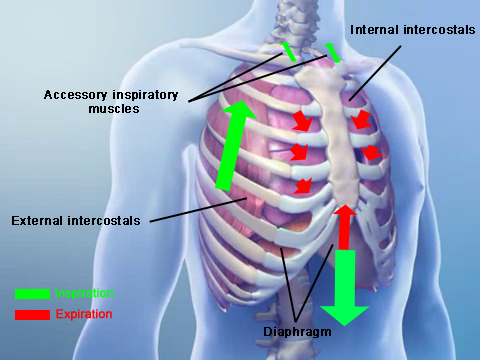
\includegraphics[height=8cm]{pics/respiratory_schema}
	\caption[Respiratory system in action]{\label{fig:respiratory_schema}Respiratory system in action. Diagram taken from the Biophysics4Arab's Channel.}
\end{figure}

During the inspiration phase of breathing the diaphragm (which is a large and thin muscle, which stretches across the chest under the rib cage separating the abdominal cavity from the chest cavity) contracts and flattens out going downward and expanding the space in the chest. The diaphragm gains its shape from its attachments and the surrounding organs: heart, lungs, and liver. At the same time, the external intercostal muscles contract pulling the rib cage upward and expanding the thoracic cavity (and as a consequence the lungs' volume). During forceful inspirations, the scalene muscles located in the neck contract to further enlarge the thoracic cavity. As the rib cage expands, the intra-alveolar pressure reduces below the atmosphere pressure. The air is drawn into the lungs until the pressure equilibrates.

During expiration the diaphragm and the intercostal muscles relax and the thoracic cavity and the lungs return to their pre-inspiratory size. As the lungs recoil the intra-alveolar pressure increases above the atmosphere pressure. The air goes out of the lungs until the pressure equilibrates again. No muscles contract during quiet expiratory breathing. However, during forceful expirations, the abdominal muscles and the internal intercostal muscles contract to reduce the thoracic cavity further than during passive expiration. The abdomen wall is indirectly driven by the pumping of the diaphragm and stores potential energy through inhalation, which could be usable for exhalation.

Interestingly enough, the lungs do not affect the outward appearance of the trunk during regular respiration \cite{zordan2004breathe}.

% -------------------------------------------------------------
% Section
% -------------------------------------------------------------
\section{\label{sec:rigid_body_component}Rigid-body components}
As the mechanism of breathing is driven by two different sections of the chest wall, our torso simulation includes three main categories: rigid-body components (e.g. spine, ribs and sternum), soft-body components (e.g. lungs, abdomen and diaphragm) and the muscle elements.
	
In contrast to DiLorenzo et al. \cite{dilorenzo2009breathing} and Veltkamp et al. \cite{veltkamp2009physiological} who used a skeleton from \url{www.3Dcafe.com} and Lee et al. \cite{lee2008biomechanical} who used the commercial Ultimate Human model, we used a skeleton of high anatomical accuracy. The partial skeleton (spine, ribs and sternum) in figure \ref{fig:skeleton} was taken from a complete 3D skeleton model constructed by Dr. M. Bobot who used real anatomical data in its construction. We are very grateful for his permission to use this skeleton.

 The skeleton, which can be seen in figure \ref{fig:skeleton}, was kindly given by Dr. M. Bobot who realised it from several anatomy books \cite{sobotta1977atlas, netter2009atlas, gray1918anatomy}. From the whole 3D skeleton model, only the vertebrae of the spine, the ribs and the sternum were used.

\begin{figure}[h]
	\centering
	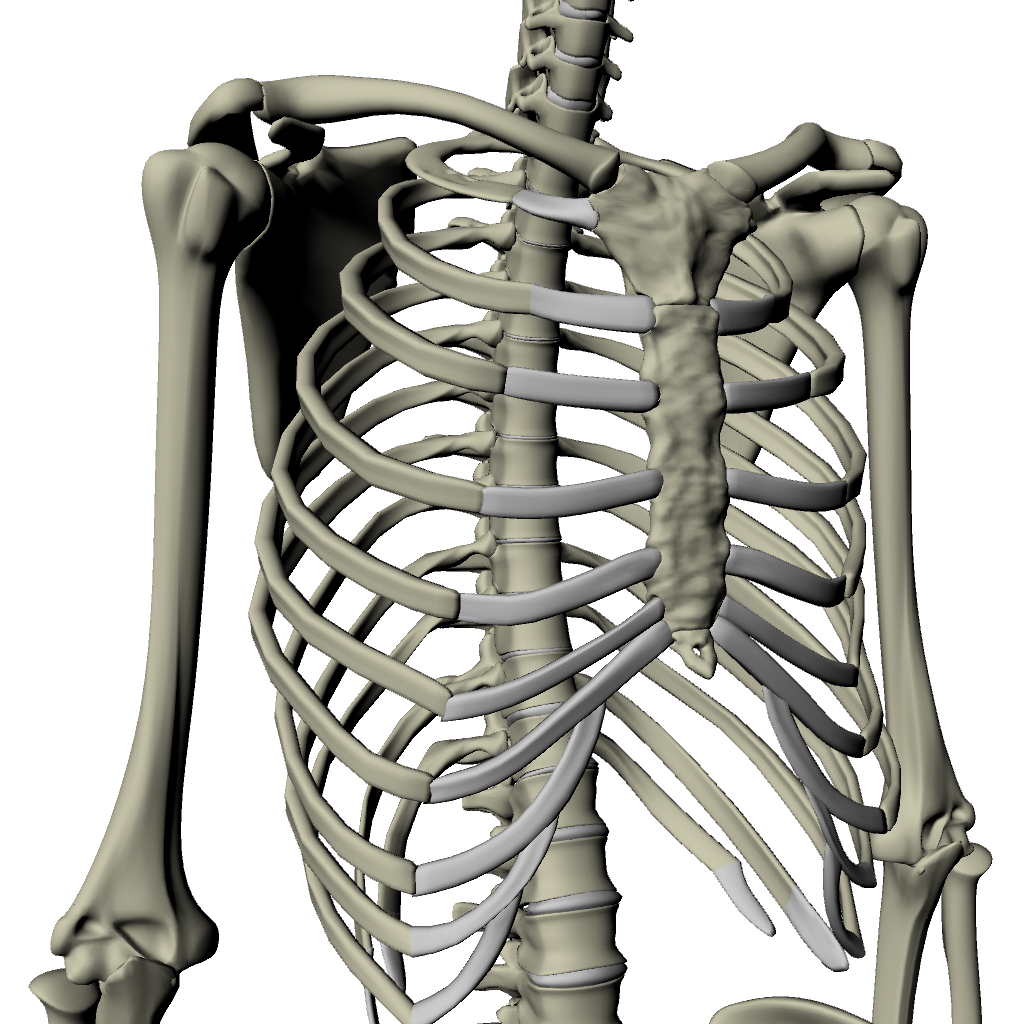
\includegraphics[height=7cm]{pics/skeleton}
	\caption[Skeleton model used]{\label{fig:skeleton}Skeleton model used.}
\end{figure}	

\subsection{\label{sec:spine}Spine}
The spine is composed of 24 vertebrae. The different regions of the vertebral column contribute to the skeletal framework of the thorax, abdomen, and pelvis. The number and specific characteristics of the vertebrae vary depending on the body region with which they are associated. There are seven cervical, twelve thoracic, five lumbar, five sacral, and three to four coccygeal vertebrae (see figure \ref{fig:spine_netter}). The spine simulation can be seen in figure \ref{fig:spine_simu}.

Between adjacent vertebrae in the spine lies an intervertebral disc. Each disc forms a cartilaginous solid joint to allow slight movement of the vertebrae, and acts as a ligament to hold the vertebrae together. As in \cite{dilorenzo2009breathing, veltkamp2009physiological, lee2008biomechanical}, we modelled each joint as a ball joint.

\begin{figure}
\centering
\subfigure[Anatomical vertebral column from \cite{netter2009atlas}.]{
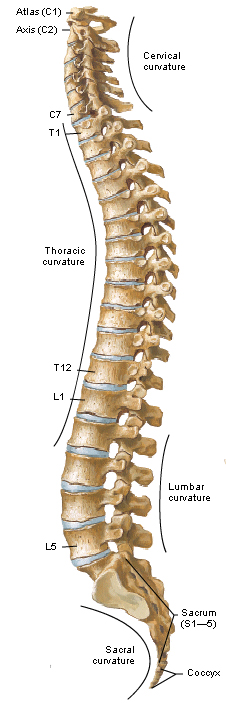
\includegraphics[width=0.4\textwidth]{pics/spine_netter}
\label{fig:spine_netter}
}
\subfigure[Simulated vertebral column.]{
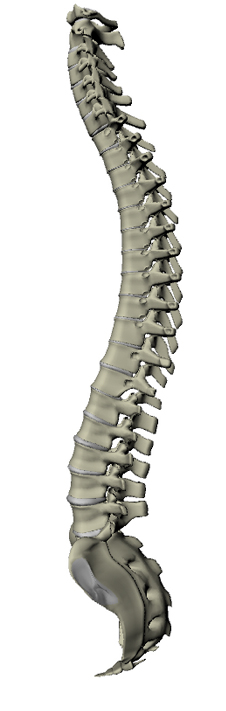
\includegraphics[width=0.4\textwidth]{pics/spine_simu}
\label{fig:spine_simu}
}
\caption[Comparison of true and simulated spine]{\label{fig:spine}Comparison of true and simulated spine.}
\end{figure}

\subsection{\label{sec:thoracic_cage}Thoracic cage}
Thanks to its shape that provides rigidity, the thoracic cage (rib cage) protects internal structures within the thorax (e.g. heart, great vessels, lungs, and trachea). The thoracic cage includes the sternum, twelve pairs of ribs (numbered from one to twelve, from top to bottom as shown in figure \ref{fig:thorax_gray}) and costal cartilages, the twelve thoracic vertebrae and intervening intervertebral discs mentioned in section \ref{sec:spine}. Because the thorax area is constantly in motion, it is one of the most dynamic regions of the body. With each breath, the muscles of the thoracic wall work in concert with the diaphragm and muscles of the abdominal wall vary the volume of the thoracic cavity. This is done first by expanding the capacity of the cavity, thereby causing the lungs to expand and draw air in and then, due to lung elasticity and muscle relaxation, decreasing the volume of the cavity and causing the lungs to expel air.

The domed shape of the thoracic cage provides remarkable rigidity, given the light weight of its components, enabling it to:
\begin{enumerate}
	\item Protect vital thoracic and abdominal organs (heart, great vessels, lungs, and trachea) from external forces.
	\item Resist the negative (sub-atmospheric) internal pressures generated by the elastic recoil of the lungs and inspiratory movements.
	\item Provide attachment for and support the weight of the upper limbs.
	\item Provide the anchoring attachment (origin) of many of the muscles that move and maintain the position of the upper limbs relative to the trunk, as well as provide the attachments for muscles of the abdomen, neck and the back.
\end{enumerate}	

The sternum and cartilage that connect to the ribs is a very stiff but deformable material. We approximate cartilage by modelling it as a rigid body. As the global movement between a rib and the sternum are mainly rotations due to the very stiff nature of the cartilage, we modelled the joint between each rib to the sternum with a ball joint. The sternum moves ventrally. Consequently, there is usually an increase in both the lateral and the dorsoventral diameters of the rib cage during inspiration.

Ribs are curved, flat bones that form most of the thoracic cage as shown in figure \ref{fig:rib_netter}. There are three types of ribs:

\begin{enumerate}
	\item True (vertebrocostal) ribs (1st-7th ribs): they attach directly to the sternum through their own costal cartilages.
	\item False (vertebrochondral) ribs (8th, 9th, and usually 10th ribs): their cartilages are connected to the cartilage of the rib above them; thus their connection with the sternum is indirect.
	\item Floating (vertebral, free) ribs (11th, 12th, and sometimes 10th ribs): the rudimentary cartilages of these ribs do not connect even indirectly with the sternum; instead they end in the posterior abdominal musculature.
\end{enumerate}	

The displacements of the rib cage during breathing are essentially due to the motion of the ribs. Each rib is fixed to the spine with two joints: the costovertebral and costotransverse joints, together resulting in a hinge joint in the direction of the rib's neck as shown in figure \ref{fig:rib_moore}. When a rib is displaced, its ventral end moves laterally and ventrally as well as cranially. The sternum moves ventrally. Consequently there is usually an increase in both the lateral and the dorsoventral diameters of the rib cage during inspiration.

We have assigned physiology based masses to these rigid components of the rib cage using data given by \cite{dilorenzo2009breathing} (see table \ref{tab:body_masses}).

\begin{table}
\begin{center}
\begin{tabular}{|c|c|}
\hline
 Body part & Mass (kg)\\ 
\hline
\hline
 Skull & 3.94 \\
 C1-C3 & 0.24 \\ 
 C4-C7 & 0.38 \\ 
 T1-T4 & 0.86 \\ 
 T5-T8 & 0.83 \\ 
 T9-T12 & 0.83 \\ 
 L1-L3 & 0.83 \\ 
 L4-L5 & 0.83 \\ 
 Rib 2 Cartilage & 0.03 \\ 
 Rib 3 Cartilage & 0.06 \\ 
 Rib 4 Cartilage & 0.08 \\
 Rib 5 Cartilage & 0.07 \\ 
 Rib Lower Cartilage & 0.47 \\ 
 Sternum & 0.58 \\ 
 Abdomen & 8 \\ 
  
\hline
\end{tabular}
\end{center}
\caption[Body masses]{\label{tab:body_masses}Body masses. Data given by \cite{dilorenzo2009breathing}.}
\end{table}

\begin{figure}
\centering
\subfigure[Rib diagram from \cite{netter2009atlas}.]{
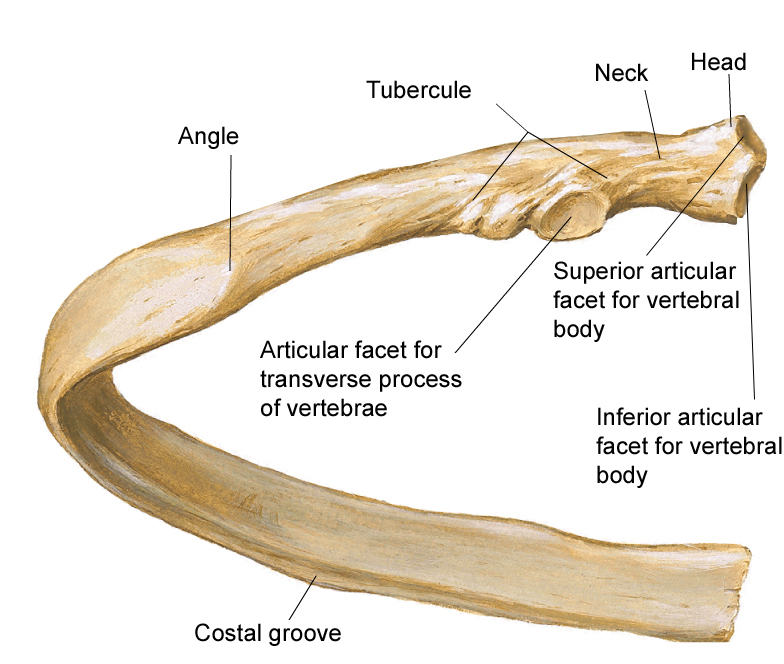
\includegraphics[width=0.7\textwidth]{pics/rib_netter}
\label{fig:rib_netter}
}
\subfigure[Costovertebral articulations of a typical rib. The rib moves (elevates and depresses) around an axis that traverses the head and the neck of the rib. This axis is oriented laterally, dorsally and caudally. Diagram taken from \cite{moore1992clinically}.]{
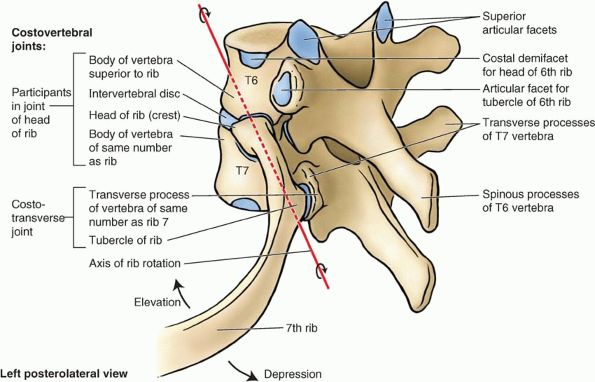
\includegraphics[width=1\textwidth]{pics/rib_moore}
\label{fig:rib_moore}
}
\caption[The different parts of an individual rib and its articulations]{\label{fig:rib}\subref{fig:rib_netter} the different parts of an individual rib and \subref{fig:rib_moore} its articulations.}
\end{figure}
		
In contrast to \cite{dilorenzo2009breathing}, who modelled the joints between each rib and the spine with ball joints and \cite{veltkamp2009physiological} who modelled them with hinge joints but only oriented laterally, our modelling is anatomically correct with hinge joints crossing the \emph{articular facet for transverse processes of vertebrae} and the middle of the \emph{superior articular facet for vertebral body} and the \emph{inferior articular facet for vertebral body} of each rib (see figure \ref{fig:rib}).
		
In figure \ref{fig:thorax} we can see a frontal view of \subref{fig:thorax_gray} an anatomical rib cage versus \subref{fig:thorax_simu} our simulated rib cage, versus \subref{fig:thorax_breathe_easy} the simulated rib cage from Breathe Easy \cite{dilorenzo2009breathing}. We notice that in the Breathe Easy simulation, the first rib is over curved in the cranial direction and that from the 4th to the 8th rib, the curvature is too high resulting in a rib cage with a wide end.

\begin{figure}[h]
\centering
\subfigure[Anatomical rib cage from \cite{netter2009atlas}.]{
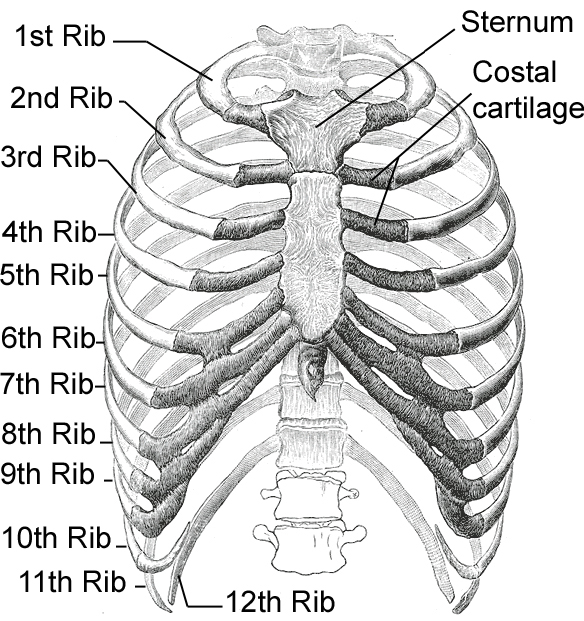
\includegraphics[width=0.3\textwidth]{pics/thorax_gray}
\label{fig:thorax_gray}
}
\subfigure[Simulated rib cage.]{
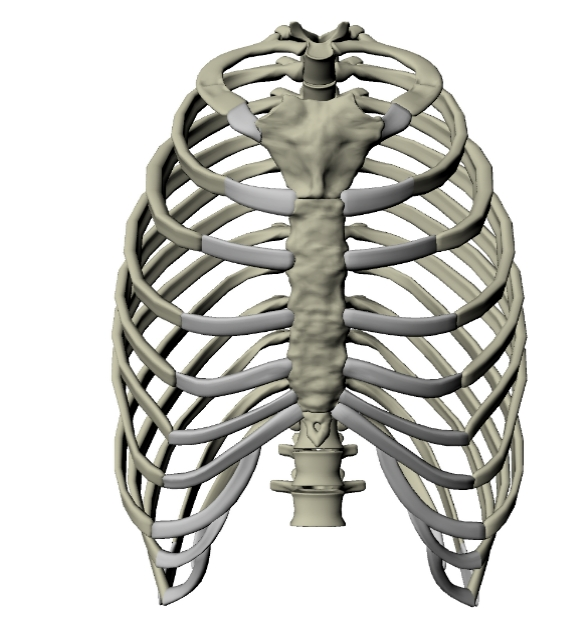
\includegraphics[width=0.3\textwidth]{pics/thorax_simu2}
\label{fig:thorax_simu}
}
\subfigure[Simulated rib cage from Breathe Easy \cite{dilorenzo2009breathing}.]{
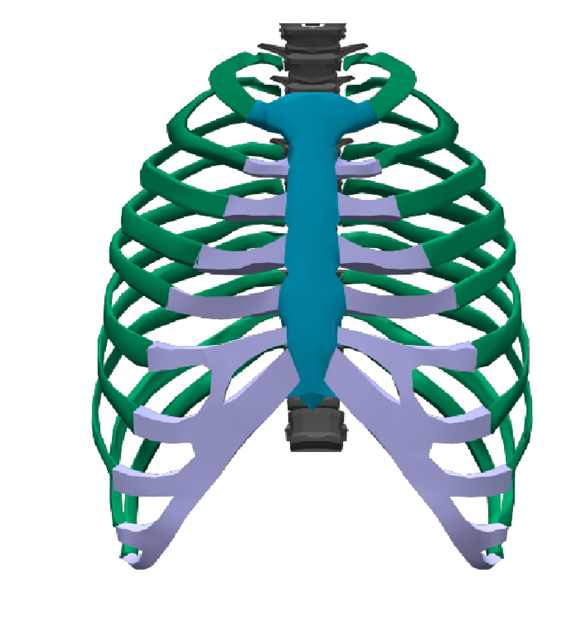
\includegraphics[width=0.3\textwidth]{pics/thorax_breathe_easy}
\label{fig:thorax_breathe_easy}
}
\caption[Comparison with the simulated rib cage]{\label{fig:thorax}Comparison with the simulated rib cage.}
\end{figure}		